\documentclass[11pt]{article}
\usepackage[margin=1in]{geometry}
\usepackage{volfit_preamble}
\graphicspath{{figures/}}

\title{\textbf{What the Optimizer Sees}\\[2pt]
\large The calibration objective as a choice of units, a measure, and a
tolerance\\[2pt]
\normalsize Vol-Fitter Technical Notes, No.~07}
\author{Vol-Fitter}
\date{\today}

\begin{document}
\maketitle

% Generated numbers.  obj_measure_tables.tex carries everything unique to
% this edition (gen_obj_measure.py).  Never retype a generated number.
% Auto-generated by gen_obj_measure.py — do not edit.
\newcommand{\objmunitserrsmall}{3.0}
\newcommand{\objmunitserrbig}{125}
\newcommand{\objmmeaserrtv}{0.062}
\newcommand{\objmmeaserreq}{0.14}
\newcommand{\objmwingratio}{1.3}
\newcommand{\objmanchor}{0.05}
\newcommand{\objmhaircut}{0.005}
\newcommand{\objmflexrigid}{6}
\newcommand{\objmflexflex}{47}
\newcommand{\objmroughmid}{0.2}
\newcommand{\objmroughband}{0.1}
\newcommand{\objmdialbandzero}{0.0}
\newcommand{\objmdialmidzero}{84}
\newcommand{\objmdialmidfull}{82}
\newcommand{\objmdialbandfull}{82}
\newcommand{\objmvalley}{126}
\newcommand{\objmrefagree}{-16}
\newcommand{\objmgencommit}{666b2dd}
\newcommand{\objmgendate}{2026-07-18}


\begin{abstract}
Every model in this series --- LQD, SVI, Multi-Core Sigmoid, local
volatility --- is calibrated by minimizing the same kind of objective, and
before any model-specific mathematics runs, three decisions have already
shaped what the optimizer can possibly find: the \emph{units} the residual
is measured in, the \emph{measure} the residuals are summed against, and
the \emph{tolerance} inside which a residual counts as zero.  This lecture
develops the shared objective as exactly those three choices.  Units: a
least-squares loss silently asserts a noise model, and the vega-normalized
price residual is the change of coordinates under which quote noise is
homogeneous --- a uniform $50$ vol bp misfit that price units squash by an
order of magnitude in the wings reads flat to \objmunitserrsmall\ vol bp
after normalization (and the dictionary is honestly local: at $300$ bp the
second-order vomma term is worth up to \objmunitserrbig\ bp in the wings).
Measure: per-quote weights are a quadrature rule --- equal weights
integrate the smile against the accident of the exchange's listing
density, while the density-corrected time-value scheme integrates against
the declared time-value measure, tracking its continuum integral to a
Kolmogorov distance of \objmmeaserrtv\ where equal weights distort it to
\objmmeaserreq.  Tolerance: the bid--ask band objective is an
$\eps$-insensitive loss whose per-quote tube is the quoted spread; alone
it has a flat valley of minimizers \objmvalley\ vol bp wide on a clean
chain, and the small mid anchor is the declared rule for selecting one
representative from it.  The band's practical value is then stated more
sharply than ``it ignores noise'': inside the tube the data term's weight
drops from $1$ to $\objmanchor$, a factor-twenty relief in the
data-versus-regularization contest --- worth \objmflexrigid\ vol bp on a
rigid model and \objmflexflex\ on a flexible one, measured on production
fits.  The reported RMS mirrors whichever objective was actually
minimized, and a haircut dial sweeps the whole construction continuously
from band back to mid.
\end{abstract}

\newpage
\tableofcontents
\newpage

%======================================================================
\section{Three decisions before any model fits}
\label{sec:three}

Strip any of this series' calibrations to its skeleton and the same object
appears: a vector of per-quote residuals, squared, weighted, summed, and
handed --- together with each model's own penalty blocks --- to a
least-squares engine.  The master data term, shared verbatim by every
model, is
\begin{equation}
\boxed{\;
\sum_i \lambda_i\Big[\big(m_i-\mathrm{hi}_i\big)_+^2
+\big(\mathrm{lo}_i-m_i\big)_+^2
+\theta_{\mathrm{mid}}\,\big(m_i-\mathrm{mid}_i\big)^2\Big],\;}
\label{eq:master}
\end{equation}
with $m_i$ the model's value at quote $i$ \emph{in the residual units},
$[\mathrm{lo}_i,\mathrm{hi}_i]$ a per-quote tolerance band (which may
collapse to the mid), $\lambda_i$ the observation weights and
$\theta_{\mathrm{mid}}$ a small anchor.  Everything in
\eqref{eq:master} that is not the model is one of three choices, and each
is a piece of applied mathematics worth a section:
\begin{itemize}[leftmargin=1.6em,itemsep=1pt]
\item \textbf{Units} (\cref{sec:units}): in what coordinates is $m_i$
measured?  A least-squares loss is a Gaussian likelihood in whatever units
its residuals live in; choosing the units \emph{is} choosing the noise
model.
\item \textbf{Measure} (\cref{sec:measure}): the sum over quotes is a
quadrature of a continuum misfit functional; the weights decide which
measure on the strike axis that quadrature approximates --- and the
exchange's listing schedule is the wrong default.
\item \textbf{Tolerance} (\cref{sec:tolerance}): a quote is an interval,
not a number; the hinge terms make the interval a zero-cost tube, and the
anchor decides which member of the tube's flat valley of minimizers is
returned.
\end{itemize}
The remaining sections measure what the tolerance is worth in a real
contest with a regularizer (\cref{sec:contest}) and insist that the
reported error mirror the objective actually minimized
(\cref{sec:honest}).  The models' own penalty blocks --- calendar floors,
wing slopes, butterfly hinges, priors --- stack into the same
least-squares vector but are documented where they belong (Notes~03, 09,
10 and 13); this note owns only the shared machinery.

\begin{invariant}
\begin{enumerate}[leftmargin=1.6em]
\item One objective vocabulary for every model: same residual units, same
weight schemes, same band construction --- a mode or scheme change means
the same thing on LQD, SVI, MCS and LV.
\item Weights are mean-normalized to one, so switching schemes never
silently re-tunes the data-versus-regularization balance.
\item Inside the quoted band the fit pays only the small mid anchor ---
the band never pushes, it only stops punishing.
\item The reported RMS is the distance to the objective that was actually
minimized, under the weights that were actually used.
\end{enumerate}
\end{invariant}

\paragraph{Conventions and the notation ledger.}
$k$ is log-moneyness, $T$ the year fraction, $\tvar=\sigma^2T$ total
implied variance, $\Black(k,\tvar)$ the normalized Black call and
$\partial_\sigma\Black=\phin(d_+)\sqrt T$ its vega.  Per quote $i$:
model value $m_i$, quoted $\mathrm{mid}_i$ and band
$[\mathrm{lo}_i,\mathrm{hi}_i]$, weight $\lambda_i$, time value
$\mathrm{TV}_i$ (the OTM option's normalized price), Voronoi cell width
$s_i$ in log-strike with mean $\bar s$.  $\theta_{\mathrm{mid}}$ is the
mid-anchor weight, $h$ the haircut in vol points, $\eta$ the vega floor,
$\eps$ a numerical floor, $\mu$ a measure on the strike axis.  One vol bp
is $10^{-4}$ of absolute volatility.  Subscripted $\partial$ for
partials; no primes.

\begin{table}[H]
\centering\footnotesize
\setlength{\tabcolsep}{4pt}
\begin{tabular}{@{}llll@{}}
\toprule
$k,\ T,\ \tvar$ & log-moneyness, expiry, total variance &
$m_i,\ \mathrm{mid}_i,\ [\mathrm{lo}_i,\mathrm{hi}_i]$ & model value; quote; band\\[2pt]
$\Black,\ \partial_\sigma\Black,\ \eta$ & Black call, vega, vega floor &
$\lambda_i,\ \mathrm{TV}_i,\ s_i,\ \bar s$ & weights; time value; cell widths\\[2pt]
$\theta_{\mathrm{mid}},\ h$ & mid anchor; haircut (vol pts) &
$\mu,\ \eps$ & strike-axis measure; floor\\[2pt]
$d_\pm$ & Black arguments &
$(x)_+$ & $\max(x,0)$\\
\bottomrule
\end{tabular}
\caption{Every symbol in the note.  Weights are $\lambda_i$, never
$\omega$ --- total variance $\tvar$ keeps sole claim to a $w$-like glyph.}
\label{tab:ledger}
\end{table}

%======================================================================
\section{Units: the residual as a change of coordinates}
\label{sec:units}

A smile is quoted in volatility but the arbitrage-free object --- for the
density models, LQD and LV --- is the \emph{price}: their parametrizations
guarantee a valid density at every iterate precisely because they live in
price space (Notes~01 and 04).  Prices, however, are terrible residual
units: the same volatility error is worth wildly different amounts of
price across moneyness.  \Cref{fig:units}A makes the point with one
experiment --- a \emph{uniform} $50$ vol bp misfit, expressed in price,
is an order of magnitude smaller in the wings than at the money.  A
least-squares loss on raw prices would therefore concentrate all its
attention at the money and let the wings drift: not because anyone chose
that, but because the units chose it.

\begin{heuristic}
A least-squares objective is the maximum-likelihood estimator for
independent Gaussian noise \emph{in the units of its residuals}.  Fitting
raw prices asserts ``quote noise is a constant number of dollars at every
strike''; fitting vols asserts ``a constant number of vol points''.  The
second is far closer to how markets quote and how desks think, so the
residual should live in vol units --- the question is how to get there
without giving up the price-space parametrizations that make arbitrage
freedom free.
\end{heuristic}

The resolution is one division.  For a quote with total variance $\tvar$
at $k$, the shared residual is
\begin{equation}
r=\frac{C^{\text{model}}(k)-\Black(k,\tvar)}
{\partial_\sigma\Black(k,\tvar)+\eta},
\label{eq:vega}
\end{equation}
the model's price error divided by Black vega, floored at $\eta$ in the
far wings.  The numerator is computed in the model's native,
arbitrage-preserving price space --- every iterate is a valid density ---
and the division is a change of coordinates:

\begin{proposition}[The dictionary, with its error term]
\label{prop:units}
Let the model and market vols at a strike differ by $\Delta\sigma$.  Then
the residual \eqref{eq:vega} satisfies
\begin{equation}
r=\Delta\sigma\Big(1+\tfrac12\,\frac{d_+d_-}{\sigma}\,\Delta\sigma
+O(\Delta\sigma^2)\Big)\quad(\eta\ \text{negligible}):
\label{eq:dict}
\end{equation}
to first order the vega-normalized price residual \emph{is} the vol
residual, uniformly across strikes; the leading correction is the
vomma-to-vega ratio $\partial^2_\sigma\Black/\partial_\sigma\Black
=d_+d_-/\sigma$, largest in the wings where $|d_\pm|$ grow.
\end{proposition}

\begin{proof}
Taylor-expand the numerator in $\sigma$:
$C^{\text{model}}-\Black=\partial_\sigma\Black\,\Delta\sigma
+\tfrac12\partial^2_\sigma\Black\,\Delta\sigma^2+\dots$, divide by
$\partial_\sigma\Black$, and use the classical
$\partial^2_\sigma\Black=\partial_\sigma\Black\,d_+d_-/\sigma$.
\end{proof}

\Cref{fig:units}B audits both halves of \cref{prop:units} on the running
smile: at a $50$ bp misfit the normalized residual is flat to
\objmunitserrsmall\ vol bp across the whole strike range --- the
dictionary in its domain --- while at $300$ bp the vomma term bends it by
up to \objmunitserrbig\ bp in the wings.  The dictionary is local, and
honestly so: during the early iterations of a cold fit the loss is only
\emph{approximately} a vol loss, converging to exactly one as the misfit
shrinks.  For the vol-space models (SVI, MCS) the residual is natively
$\Delta\sigma$ and \eqref{eq:vega} degenerates to exactly that: one
residual concept, two implementations, identical units (invariant~1).
The floor $\eta$ is the deliberate exception to the dictionary: where
vega falls below it --- strikes several standard deviations out --- the
denominator stops shrinking, which caps the vol-amplification of a price
error and quietly down-weights quotes whose vol content is numerically
vacuous.

\begin{figure}[H]
\centering
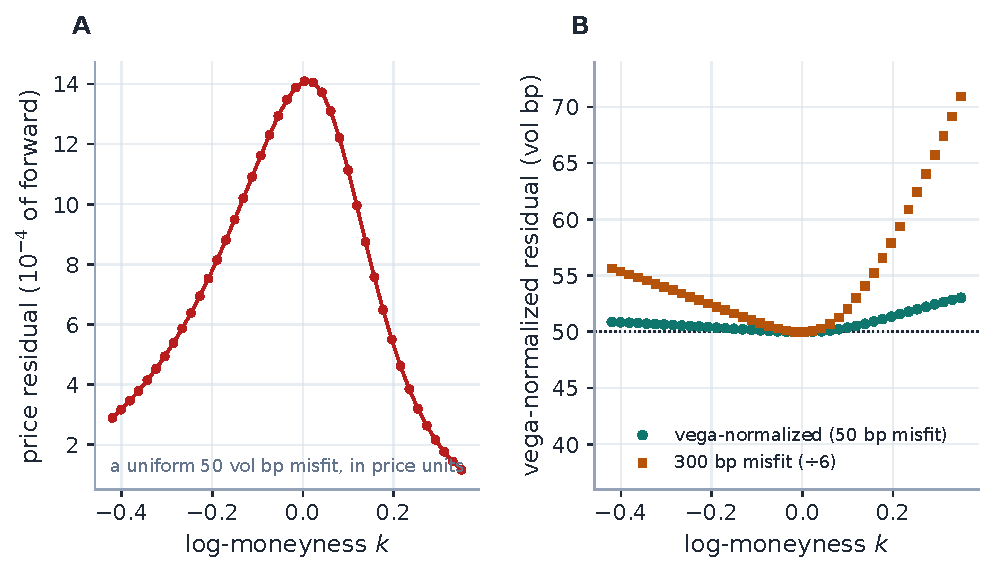
\includegraphics[width=\textwidth]{fig_objm_units.pdf}
\caption{The change of units, audited (production Black machinery, running
smile).  A: a \emph{uniform} $50$ vol bp misfit expressed in price units
--- the bell of vega: a raw-price loss would see the wings at a tenth of
their true size.  B: the same misfit after vega normalization
\eqref{eq:vega} reads flat at $50$ bp to \objmunitserrsmall\ bp (teal);
a $300$ bp misfit (rust, scaled $\div6$ for display) bends away from the
dictionary by up to \objmunitserrbig\ bp in the wings --- the vomma term
of \cref{prop:units}, the price of using a first-order dictionary far
from the optimum.}
\label{fig:units}
\end{figure}

\paragraph{Exercise 1.}
Evaluate the correction in \eqref{eq:dict} at the left edge of
\cref{fig:units} ($k=-0.42$, $\sigma\approx28\%$, $T=0.5$, so
$d_+d_-/\sigma\approx7$) for $\Delta\sigma=0.03$, and check the order of
magnitude against the measured \objmunitserrbig\ vol bp.  Then explain why
the same computation at $\Delta\sigma=0.005$ predicts a deviation below
$5$ bp --- and why an optimizer that starts within a few hundred bp of the
truth therefore feels an almost exactly vol-metric loss for its entire
descent.

%======================================================================
\section{Measure: weights as a quadrature rule}
\label{sec:measure}

\subsection{What a sum over quotes integrates}

Idealize the fit as a continuum problem: minimize
$\int\big(m(k)-\text{market}(k)\big)^2\,\dd\mu(k)$ for some measure $\mu$
on the strike axis.  Any finite quote set turns the integral into a sum,
and the weights $\lambda_i$ are the quadrature rule.  Equal weights make
$\mu$ the \emph{empirical measure of the listing} --- the exchange's
strike schedule, dense at the money, sparse in the wings.  That measure
was chosen by a listings committee, not by anyone's view of where smile
errors matter: a tight ATM cluster of near-duplicate quotes outvotes an
isolated wing quote by sheer count, and the fit follows the sampling
accident.

The desk's declared measure is different: strike ranges should matter in
proportion to the \emph{time value} they carry ---
$\dd\mu=\mathrm{TV}(k)\,\dd k$, economic content times length.  The
production scheme implements precisely the midpoint quadrature of that
measure:
\begin{equation}
\lambda_i\;\propto\;\max(\mathrm{TV}_i,\eps)\;\frac{s_i}{\bar s},
\label{eq:tvweights}
\end{equation}
where $s_i$ is quote $i$'s one-dimensional Voronoi cell width in
log-strike --- half the gap to each neighbour, one-sided at the ends: the
stretch of strike axis this quote alone represents.

\begin{proposition}[The weights are a quadrature]
\label{prop:quad}
For any smooth integrand $f$,
$\sum_i \mathrm{TV}_i\,s_i\,f(k_i)$ is the midpoint-type Riemann sum of
$\int \mathrm{TV}(k)f(k)\,\dd k$ over the Voronoi partition; in
particular the weighted loss with \eqref{eq:tvweights} discretizes the
continuum time-value objective, up to the global normalization.  On a
uniform grid all $s_i$ are equal, $s_i/\bar s=1$, and
\eqref{eq:tvweights} reduces to the pure time-value weighting
$\lambda_i\propto\mathrm{TV}_i$ --- there is no double-counting left to
correct.
\end{proposition}

\begin{proof}
The cells $\{s_i\}$ partition the quoted interval and $k_i$ lies in cell
$i$, so the sum is a Riemann sum over that partition; refinement
convergence is the standard statement.  The uniform-grid case is
arithmetic.
\end{proof}

Two guard rails keep the quadrature honest on real ladders.  The cell
width of an isolated far-wing quote is unbounded, so the spacing
multiplier $s_i/\bar s$ is capped (at $10\times$): beyond the cap the
scheme deliberately \emph{under}-integrates the deep wing rather than let
one quote carry a tenth of the objective.  And the final weights are
mean-normalized to one --- a scaling detail with a design consequence:
every regularizer in the series (the LQD ridge, the MCS hat ridge, the LV
roughness penalty) is tuned against unit-mean data weights, so switching
schemes re-\emph{distributes} the data term without re-\emph{scaling} it,
and the data-versus-regularization balance survives untouched
(invariant~2).

\subsection{The audit}

\Cref{fig:measure} runs the production weights on a realistic ladder ---
a dense ATM cluster flanked by sparse wings.  Panel A is the per-quote
view: the clustered quotes are individually down-weighted, the sparse
wing quotes up-weighted (the largest wing weight is
$\objmwingratio\times$ the ATM one).  Panel B is the measure-level audit
this edition adds: the \emph{cumulative} weight across the strike axis,
compared with the continuum time-value integral it is supposed to
discretize.  The density-corrected scheme tracks the continuum to a
Kolmogorov distance of \objmmeaserrtv; equal weights distort the measure
to \objmmeaserreq\ --- pushed above the target through the cluster,
starved in the wings.  A fit is an average against a measure; panel B
shows which measure each scheme actually supplies.

\begin{figure}[H]
\centering
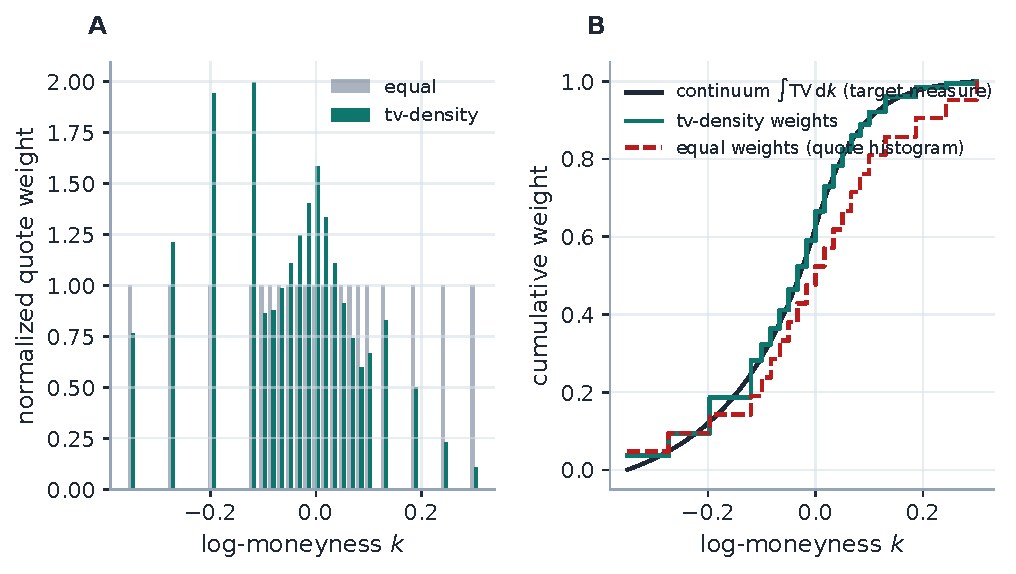
\includegraphics[width=\textwidth]{fig_objm_measure.pdf}
\caption{Weights as quadrature (production weights, realistic ladder).
A: per-quote weights --- the dense ATM cluster down-weighted, sparse
wings up-weighted, wing-to-ATM ratio $\objmwingratio$.  B: the
measure-level audit: cumulative weight against the continuum time-value
integral (black).  The density-corrected scheme (teal) is a faithful
quadrature of the declared measure (Kolmogorov distance \objmmeaserrtv);
equal weights (rust) integrate against the listing histogram instead
(\objmmeaserreq) --- the fit inherits the exchange's strike schedule as
an accidental prior.}
\label{fig:measure}
\end{figure}

\paragraph{Exercise 2.}
On \cref{fig:measure}'s ladder, thirteen of twenty-one quotes sit in
$|k|\le0.10$.  Compute the fraction of total weight the equal scheme
assigns that interval, and compare with the time-value measure's fraction
(read both off panel B).  Conclude in one sentence why adding \emph{more}
ATM listings --- which adds information --- would make an equal-weighted
fit \emph{worse} in the wings, and why that paradox disappears under
\eqref{eq:tvweights}.

%======================================================================
\section{Tolerance: the band, the tube, and the anchor}
\label{sec:tolerance}

\subsection{A quote is an interval}

A mid pretends a price is known exactly; the market's actual statement is
an interval, $[\mathrm{bid},\mathrm{ask}]$, and any curve inside it is
consistent with the quote.  The band terms of \eqref{eq:master} encode
exactly that: a two-sided squared hinge that vanishes identically inside
the band and grows quadratically outside, plus a small anchor.  Readers
from machine learning will recognize the construction: it is the
(squared) $\eps$-insensitive loss of support-vector regression
\cite{Vapnik1998}, with the tube half-width set per quote by the market
itself --- the half-spread --- rather than by a global hyperparameter.
Equivalently, it is the log-likelihood shape of an interval-censored
observation: inside the interval, all values are equally credible.

Three modes span the construction.  \emph{Mid}: the band collapses,
$\mathrm{lo}=\mathrm{hi}=\mathrm{mid}$, and \eqref{eq:master} reduces to
weighted least squares on mids.  \emph{Bid--ask}: the raw quoted band.
\emph{Haircut}: each side is pulled toward mid by $h$ vol points, never
crossing it,
\begin{equation}
\mathrm{lo}=\min(\mathrm{bid}+h,\mathrm{mid}),\qquad
\mathrm{hi}=\max(\mathrm{mid},\mathrm{ask}-h),
\label{eq:haircut}
\end{equation}
so a quote tighter than $2h$ collapses gracefully to a mid fit on that
strike.  One dial therefore spans the whole spectrum: tight ATM spreads
behave as mids (the fit follows them exactly where they are informative)
while wide wing spreads keep a live tolerance.  The hinge is monotone in
the quote value, so the same construction works unchanged in any monotone
residual space --- implied vol for SVI/MCS, vega-normalized price for
LQD/LV --- and its subgradient is a sign, which is what plugs it into
every model's analytic Jacobian.  Both are one line each, and the
listings are verbatim production (\cref{app:ref} states the verified
agreement):

\begin{lstlisting}[caption={The two-sided band hinge and its subgradient
(from \texttt{calib/band.py}; verified identical to production).},
label={lst:band}]
def band_violation(model, lo, hi):   # > 0 only outside [lo, hi]; 0 inside
    return np.maximum(model - hi, 0.0) + np.maximum(lo - model, 0.0)

def band_violation_sign(model, lo, hi):   # +1 above, -1 below, 0 inside
    return np.where(model > hi, 1.0, 0.0) - np.where(model < lo, 1.0, 0.0)
\end{lstlisting}

\Cref{fig:tube} draws what one quote contributes under each mode: the mid
parabola, the flat-bottomed tube of the hinge alone, and the production
band loss whose interior is not perfectly flat but a parabola scaled by
$\theta_{\mathrm{mid}}=\objmanchor$ --- twenty times gentler than the
mid mode's.

\begin{figure}[H]
\centering
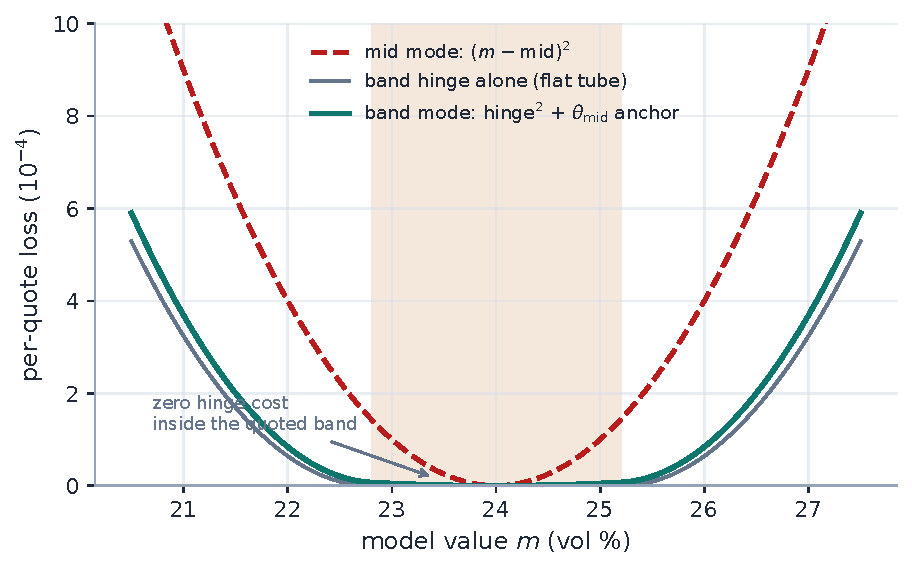
\includegraphics[width=0.82\textwidth]{fig_objm_tube.pdf}
\caption{One quote's loss under the three constructions (production
residuals).  The mid mode is a full-strength parabola; the hinge alone is
a flat zero-cost tube over the quoted band; the shipped band mode adds
the $\theta_{\mathrm{mid}}=\objmanchor$ anchor --- a parabola twenty
times shallower inside the tube, steepening to hinge strength outside.
The band never pushes the fit anywhere; it only stops punishing it
(invariant~3).}
\label{fig:tube}
\end{figure}

\subsection{The flat valley, and who selects from it}

The hinge alone has a defect a lecture should exhibit rather than paper
over: its minimizer is not a point.

\begin{proposition}[The tube's null set]
\label{prop:valley}
With $\theta_{\mathrm{mid}}=0$, the set of observation vectors minimizing
the band terms of \eqref{eq:master} is the product of intervals
$\prod_i[\mathrm{lo}_i,\mathrm{hi}_i]$: every curve lying inside every
quoted band attains the same (zero) data cost.  Any strictly positive
$\theta_{\mathrm{mid}}$ restores strict convexity in the observation
space and selects the unique mid-closest member.
\end{proposition}

\begin{proof}
Inside all bands both hinges vanish, so the data cost is zero on the
product set and positive outside it; the anchor term is a strictly convex
quadratic, and the sum of a convex function and a strictly convex one is
strictly convex.
\end{proof}

This is Note~04's equivalence-class situation in miniature: the data
(here, deliberately weakened data) does not single out an answer, so the
objective must \emph{declare} its representative, and
$\theta_{\mathrm{mid}}$ is that declaration --- of all curves the market
tolerates, return the one nearest the mids.  \Cref{fig:anchor} measures
the valley on a clean production fit: level-shifting the fitted curve,
the hinge-only cost is exactly flat over a \objmvalley-vol-bp-wide
interval --- every shift in it keeps the curve inside every band ---
while the anchored objective is a clean strictly convex bowl through the
same region.  An optimizer given the flat version stalls wherever it
first enters the tube, and \emph{where} it enters depends on the seed:
the anchor is what makes band fits reproducible.

\begin{figure}[H]
\centering
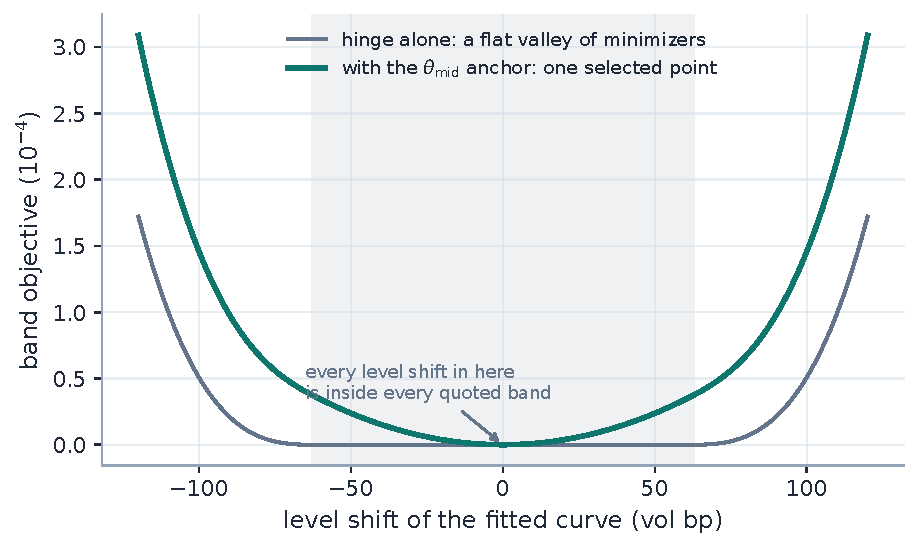
\includegraphics[width=0.82\textwidth]{fig_objm_anchor.pdf}
\caption{The tube's flat valley, measured (production band residuals on a
clean chain; the fitted curve is level-shifted through the bands).
Hinge alone: a \objmvalley\ vol bp plateau of exact minimizers --- the
null set of \cref{prop:valley}, where the answer would be
seed-dependent.  With the $\theta_{\mathrm{mid}}$ anchor: one strictly
convex bowl, one declared representative --- the mid-closest curve the
bands allow.}
\label{fig:anchor}
\end{figure}

\paragraph{Exercise 3.}
From \eqref{eq:master}, compute how far beyond a band edge the fit will
sit when something else (a regularizer, a neighbouring quote) pulls it
outward with the strength of a full mid residual of size $\delta$: balance
the hinge gradient against $\theta_{\mathrm{mid}}$ times the anchor
gradient and show the concession is
$O(\theta_{\mathrm{mid}}\,\delta)$ --- a twentieth of what the mid mode
would concede.  The band is soft, but twenty times harder than the pull
toward mid.

%======================================================================
\section{What the tolerance is worth: the contest with the regularizer}
\label{sec:contest}

It is tempting to summarize the band as ``the fit ignores noise inside
the spread'', and the temptation should be resisted, because it is not
what \eqref{eq:master} says.  Inside the tube the data term does not
vanish --- it survives at weight $\theta_{\mathrm{mid}}$.  The precise
statement is a re-weighting: \emph{entering the band divides the data
term's strength by $1/\theta_{\mathrm{mid}}=20$ in its contest with
everything else in the objective}.  Whether that relief buys anything
depends on who the ``everything else'' is:

\begin{itemize}[leftmargin=1.6em,itemsep=1pt]
\item A \emph{rigid} model is its own regularizer: it cannot chase
quote-frequency noise in any mode, so mid and band fits nearly coincide
--- measured at \objmflexrigid\ vol bp apart on the running example
(\cref{fig:flex}A).
\item A \emph{flexible} model with a live smoothness penalty is where the
tolerance earns its keep: in mid mode the full-weight residuals overrule
the regularizer and the fit tracks the tick bounce; in band mode the
regularizer wins inside the tube and the curve cuts smoothly through ---
the two fits separate by \objmflexflex\ vol bp, with the roughness of
the mid fit at $\objmroughmid$ against the band fit's $\objmroughband$
(\cref{fig:flex}B).
\item A flexible model with \emph{no} counterforce gains nothing: inside
the tube the anchor is the only force left, and the anchor points at the
mids --- the band fit returns to the noise it was meant to ignore.  The
tolerance does not smooth; it \emph{liberates whatever smooths}.
\end{itemize}

The band is still fairly called a regularizer that costs no bias --- it
pushes the fit nowhere it was not already going --- but its mechanism is
the re-weighting above, and the measured factor-eight gap between the
rigid and flexible rows is the honest size of the effect.

\begin{figure}[H]
\centering
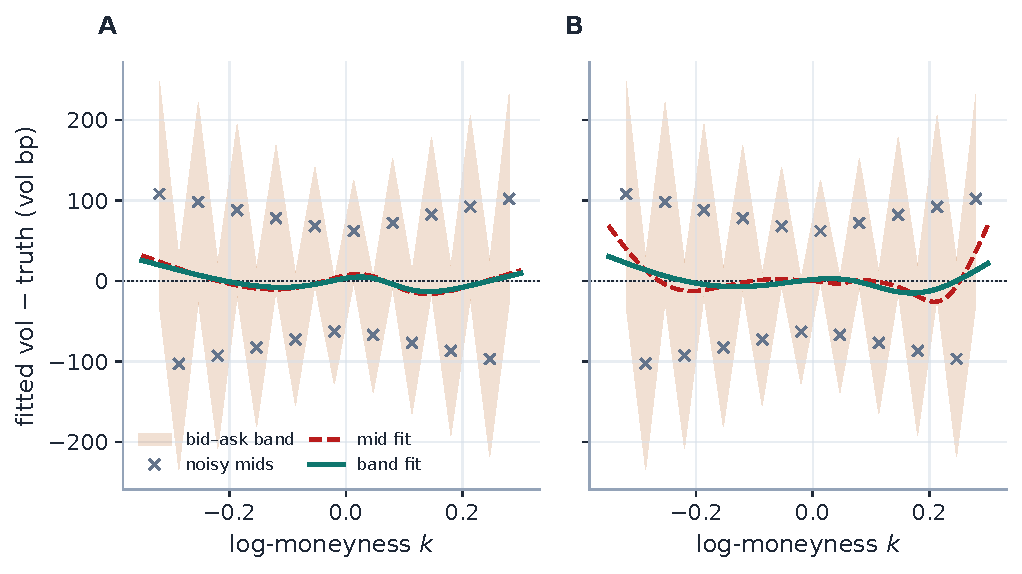
\includegraphics[width=\textwidth]{fig_objm_flex.pdf}
\caption{The contest, measured (production LQD fits; alternating
tick-bounce mids inside a wing-widening band; everything shown as
deviation from the true smile).  A: a rigid model smooths in either mode
--- mid and band fits are \objmflexrigid\ vol bp apart.  B: a flexible
model with a live ridge: the mid fit (rust) bends toward the bounce,
the band fit (teal) lets the ridge win inside the tube --- the fits
separate by \objmflexflex\ vol bp.  The band's value is exactly the
counterforce it liberates.}
\label{fig:flex}
\end{figure}

%======================================================================
\section{The honest metric, and the dial that connects the modes}
\label{sec:honest}

A reported fit error should measure the objective that was minimized,
not a decorative quantity.  The production RMS therefore mirrors the
active configuration exactly: distance to mid in mid mode; band
\emph{violation} in the band modes (a fit sitting contentedly inside the
tube reports near-zero error however far it is from the mids); the
active weights $\lambda_i$ throughout; returned as the pair
$(\sum\lambda r^2,\sum\lambda)$ so per-expiry numbers pool correctly
into a surface RMS (invariant~4).  The same fitted curve can then
legitimately print different numbers under different modes ---
\cref{fig:dial} shows the whole story on one axis by sweeping the
haircut $h$ of \eqref{eq:haircut}.  At $h=0$ (raw band) the fit is free
inside the tube: band-metric \objmdialbandzero\ vol bp, while its
distance to the noisy mids is \objmdialmidzero.  As $h$ grows the tube
tightens strike by strike, the band metric climbs, and at full collapse
both metrics agree at \objmdialbandfull\ bp: the haircut is one dial
that sweeps the objective --- and its honest metric with it ---
continuously from band fitting back to mid fitting.

\begin{figure}[H]
\centering
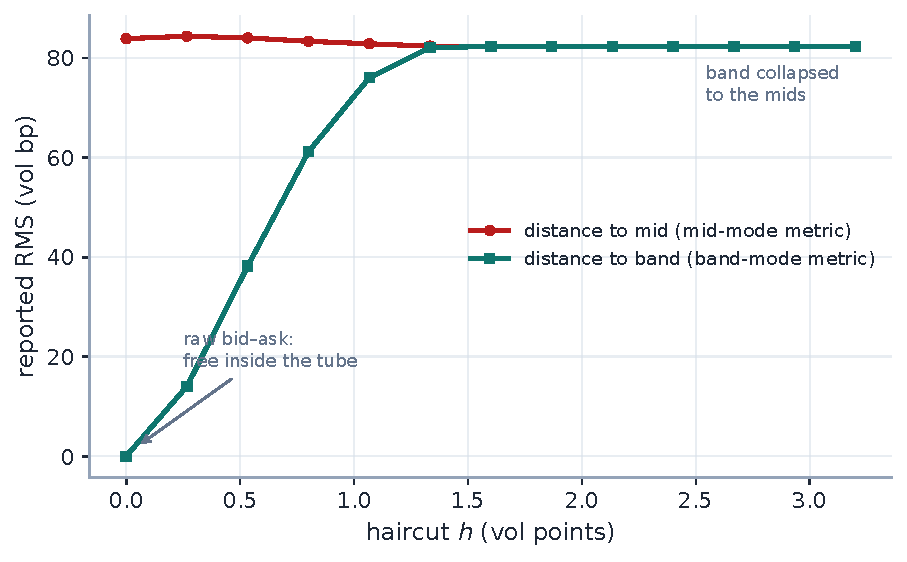
\includegraphics[width=0.82\textwidth]{fig_objm_dial.pdf}
\caption{The haircut dial and the honest metric (production fits and
production RMS at every point).  Sweeping $h$ from raw bid--ask to full
collapse: the fitted curve barely moves (its distance to mid stays near
\objmdialmidzero\ vol bp throughout) but the \emph{reported} error runs
from \objmdialbandzero\ to \objmdialbandfull\ bp as the metric follows
the objective.  Two lessons: the dial connects the modes continuously,
and an RMS quoted without its mode is not a number.}
\label{fig:dial}
\end{figure}

%======================================================================
\section{What is genuinely original here}
\label{sec:original}

Vega normalization is standard practice; the contributions are the
framings made exact and the two constructions built on them:
\begin{enumerate}[leftmargin=1.6em]
\item the \emph{density-corrected time-value weighting}
\eqref{eq:tvweights}, separating economic importance (time value) from
sampling density (the Voronoi widths) --- a declared quadrature of a
declared measure, audited against its continuum target in
\cref{fig:measure} --- with the mean-one normalization that keeps every
model's regularization invariant across schemes;
\item the \emph{space-agnostic squared-hinge band} with its monotone
subgradient, making bid--ask fitting a first-class mode of every model's
analytic Jacobian rather than a bolt-on --- and its anchor understood as
the selection rule for the tube's null set (\cref{prop:valley});
\item the \emph{sharpened account of the band's value} as a
factor-$1/\theta_{\mathrm{mid}}$ relief in the data-versus-regularization
contest, measured on production fits rather than asserted
(\cref{sec:contest}).
\end{enumerate}
Together the weights and the band let the desk say ``fit what matters,
to within the spread'' in two orthogonal dials.

%======================================================================
\section{Limitations}
\label{sec:limits}

Where the design's guarantees stop.  The objective carries \emph{no
robust loss}: outside the band the hinge grows quadratically, so a
single insane quote retains full quadratic leverage --- by design, the
defence against outliers lives upstream, in the data layer's screens and
quarantines (Notes~05 and 06), not in the loss.  The Gaussian reading of
least squares is a choice, not a fact about markets; so is the
time-value measure --- a vega-squared measure is equally defensible and
one model family carries it internally --- and declaring the measure is
the point, not deriving it.  The quadrature is truncated: the spacing
cap deliberately under-weights isolated deep-wing quotes, trading
fidelity to the declared measure for robustness to listing accidents.
The dictionary of \cref{prop:units} is first order, and a cold fit
starting far from the truth descends a loss that is only approximately
vol-metric.  And the band's value is contingent (\cref{sec:contest}): it
liberates a counterforce it does not supply, so a flexible model fitted
in band mode \emph{without} a live regularizer inherits the mids' noise
through the anchor --- tolerance is not smoothness.

\appendix
%======================================================================
\section{Hyperparameter atlas}
\label{app:atlas}

\begin{longtable}{p{0.26\textwidth}p{0.14\textwidth}p{0.52\textwidth}}
\caption{Calibration-objective hyperparameters.}\label{tab:atlas}\\
\toprule Knob & Default & Role\\ \midrule
\endfirsthead \toprule Knob & Default & Role\\ \midrule \endhead
\multicolumn{3}{l}{\emph{Surfaced (FitSettings / OptionsSettings)}}\\ \midrule
\texttt{weightScheme} & \texttt{equal} & \texttt{equal} or
\texttt{tv\_density} \eqref{eq:tvweights}.\\
\texttt{fitMode} & \texttt{mid} & \texttt{mid} / \texttt{bidask} /
\texttt{haircut}.\\
\texttt{haircut} $h$ & $\objmhaircut$ & Haircut in vol points (each band
side toward mid), \eqref{eq:haircut}.\\
\texttt{midAnchorWeight} $\theta_{\mathrm{mid}}$ & $\objmanchor$ & Mid
anchor strength vs the unit hinge.\\
\midrule
\multicolumn{3}{l}{\emph{Hidden}}\\ \midrule
\texttt{DEFAULT\_MAX\_MULT} & $10$ & Cap on the Voronoi spacing
multiplier $s_i/\bar s$ (truncated quadrature).\\
$\eps$ & $10^{-12}$ & Floor on time value / spacing.\\
$\eta$ (vega floor) & $10^{-4}$ & Floor on Black vega in
\eqref{eq:vega}.\\
\bottomrule
\end{longtable}

\noindent\textbf{Performance.}  Weighting is $O(m\log m)$ (one sort); the
band residual and its subgradient are $O(m)$ and analytic, adding nothing
to Jacobian assembly.  Both are negligible against any fit.  Switching a
scheme or mode bumps the options version and triggers exactly one refit.

%======================================================================
\section{Traceability}
\label{app:trace}

\begingroup
\small
\setlength{\tabcolsep}{4pt}
\renewcommand{\arraystretch}{1.15}
\begin{longtable}{@{}p{0.42\textwidth}p{0.10\textwidth}p{0.44\textwidth}@{}}
\caption{Claims in this note and the code/tests that lock them.}\label{tab:trace}\\
\toprule Claim & Object & Code anchor \newline \emph{Test anchor}\\ \midrule
\endfirsthead
\toprule Claim & Object & Code anchor \newline \emph{Test anchor}\\ \midrule
\endhead
Density-corrected weights match the design note's worked example &
\eqref{eq:tvweights} &
\nolinkurl{volfit/calib/weights.py}\newline
\nolinkurl{tests/test_weights.py::test_doc_worked_example}\\
\addlinespace
Uniform grid reduces to pure time value &
\cref{prop:quad} &
\nolinkurl{volfit/calib/weights.py}\newline
\nolinkurl{tests/test_weights.py::test_uniform_grid_reduces_to_time_value}\\
\addlinespace
Dense cluster down-weighted; mean-one normalization &
\eqref{eq:tvweights} &
\nolinkurl{volfit/calib/weights.py}\newline
\nolinkurl{tests/test_weights.py::test_dense_region_downweighted};
\nolinkurl{::test_resolve_weights_equal_is_none_and_tv_is_mean_one}\\
\addlinespace
The scheme moves every model (shared vocabulary) &
invariant~1 &
\nolinkurl{volfit/calib/weights.py}\newline
\nolinkurl{tests/test_weights.py::test_weight_scheme_moves_every_model}\\
\addlinespace
Band modes; haircut collapses gracefully to mid &
\eqref{eq:haircut} &
\nolinkurl{volfit/calib/band.py}\newline
\nolinkurl{tests/test_band_fit.py::test_resolve_band_modes};
\nolinkurl{::test_haircut_default_is_half_vol_point}\\
\addlinespace
Zero residual inside the band; edge pull outside &
\eqref{eq:master} &
\nolinkurl{volfit/calib/band.py}\newline
\nolinkurl{tests/test_band_fit.py::test_band_residuals_zero_inside_band};
\nolinkurl{::test_outside_band_mid_is_pulled_to_edge}\\
\addlinespace
Band fit stays in band and smooths (the contest) &
\cref{sec:contest} &
\nolinkurl{volfit/calib/band.py}\newline
\nolinkurl{tests/test_band_fit.py::test_band_fit_stays_in_band_and_smooths}\\
\addlinespace
RMS mirrors the minimized objective &
\cref{sec:honest} &
\nolinkurl{volfit/calib/rms.py}\newline
\nolinkurl{tests/test_rms.py::test_mid_mode_is_weighted_rms_distance_to_mid};
\nolinkurl{::test_band_mode_zero_inside_band_distance_outside}\\
\addlinespace
Band-mode RMS never exceeds mid-mode; surface pooling; weights bias the
RMS &
\cref{sec:honest} &
\nolinkurl{volfit/calib/rms.py}\newline
\nolinkurl{tests/test_rms.py::test_band_mode_rms_not_above_mid_mode};
\nolinkurl{::test_surface_rms_pools_expiries};
\nolinkurl{::test_weights_bias_the_rms}\\
\bottomrule
\end{longtable}
\endgroup

%======================================================================
\section{Reference implementation: the band residual stack}
\label{app:ref}

The full data term stacks two blocks per quote: the band violation
(scaled by the per-quote weight, or $1/\text{vega}$ in the LQD/LV price
space) and the weak mid anchor, so squaring and summing reproduces
\eqref{eq:master}.  All three listings in this note ---
\texttt{band\_violation}, \texttt{band\_violation\_sign}
(\cref{lst:band}) and \texttt{band\_residuals} below --- were executed
against their production counterparts by this edition's generator on
every run: agreement to $10^{\objmrefagree}$ (floating-point identity).

\begin{lstlisting}[caption={The stacked band-objective residual (distilled
from \texttt{calib/band.py}).}]
def band_residuals(model, lo, hi, mid, scale, mid_anchor_weight):
    viol = scale * band_violation(model, lo, hi)         # push inside the bid/ask band
    anchor = np.sqrt(mid_anchor_weight) * scale * (model - mid)   # weak pull to mid
    return np.concatenate([viol, anchor])                # least-squares stack (length 2N)
\end{lstlisting}

\begin{thebibliography}{9}
\bibitem{tvweights} Vol-Fitter Technical Note, \emph{Density-corrected
time-value weights}
(\texttt{Docs/iv\_time\_value\_density\_weights.tex}).
\bibitem{Gatheral2006} J.~Gatheral.  \emph{The Volatility Surface}.
Wiley, 2006.
\bibitem{Vapnik1998} V.~Vapnik.  \emph{Statistical Learning Theory}.
Wiley, 1998.  (The $\eps$-insensitive loss.)
\bibitem{Huber1981} P.~Huber.  \emph{Robust Statistics}.  Wiley, 1981.
\end{thebibliography}

\end{document}
